% Latex template: https://github.com/mqTeXUsers/Macquarie-University-Beamer-Theme

% Slide Masters:

% Title
% Text
% 2 column
% Full-image
% Bibliography
% Closing
 
\documentclass[aspectratio=169, 11pt]{beamer} % Aspect ratio
% https://tex.stackexchange.com/a/14339/5483 
% Possible values: 1610, 169, 149, 54, 43 and 32.
% 169 = 16:9

\PassOptionsToPackage{table}{xcolor}    %https://tex.stackexchange.com/a/5365/5483

\usetheme{macquarie}
\usepackage{multicol} % https://tex.stackexchange.com/a/396018/5483
\usepackage{xurl}
\usepackage[british]{babel}       % Set language
% \usepackage[utf8x]{inputenc}      % Set encoding
\usepackage{colortbl}
\mode<presentation>           % Set options
{
  \usetheme{default}          % Set theme
  \usecolortheme{default}         % Set colors
  \usefonttheme{default}          % Set font theme
  \setbeamertemplate{caption}[numbered] % Set caption to be numbered
}

% Uncomment this to have the outline at the beginning of each section highlighted.
%\AtBeginSection[]
%{
%  \begin{frame}{Outline}
%    \tableofcontents[currentsection]
%  \end{frame}
%}

\usepackage{graphicx}         % For including figures
\usepackage{booktabs}         % For table rules
\usepackage{hyperref}         % For cross-referencing


\usepackage{enumitem} % https://tex.stackexchange.com/a/2292/5483

%https://tex.stackexchange.com/a/371844/5483
\setbeamerfont{bibliography entry author}{size=\tiny}
\setbeamerfont{bibliography entry title}{size=\tiny}
\setbeamerfont{bibliography entry location}{size=\tiny}
\setbeamerfont{bibliography entry note}{size=\tiny}
\setbeamerfont{bibliography item}{size=\tiny}

% https://tex.stackexchange.com/q/333587/5483
% Uncomment to add OSF URI to each slide
% \setbeamertemplate{footline}{\strut~\texttt{https://osf.io/v5jp7/}\hfill\insertframen%umber~/~\inserttotalframenumber\strut~~~}

\usepackage{comment} % for commenting out multiple lines; uses \begin{comment} ... \end{comment}

\title{Carpentries Training at Macquarie University} % Presentation title
\author{A/Prof Shawn A Ross, Director of Data Science and eResearch}               % Presentation author
\institute{Office of the Deputy Vice-Chancellor (Research)}         % Author affiliation
\date{Thursday 14 November 2019} % Presentation date   
\begin{document}

% Title page
% This page includes the information defined earlier including title, author/s, affiliation/s and the date
% \begin{frame}[noframenumbering]

\maketitle

  
% \end{frame}

% Outline
% This page includes the outline (Table of content) of the presentation. All sections and subsections will appear in the outline by default.
\begin{frame}{The context of Research Data Management}
  \tableofcontents
\end{frame}

% The following is the most frequently used slide types in beamer
% The slide structure is as follows:
%
%\begin{frame}{<slide-title>}
% <content>
%\end{frame}


% Presentation providing context for the new data governance policies and procedures at Macquarie University

\section{Why Carpentries training?}

\begin{frame}{Data sharing in the NHMRC Statement}
    The NHMRC `strongly encourages' data sharing in the National Statement on Ethical Conduct in Human Research and their Open Access Policy. \cite{Nhmrc2018-sj, Nhmrc2018-vn} \par
    National Statement 3.1.50 \par
    In the absence of justifiable ethical reasons (such as respect for cultural ownership or unmanageable risks to the privacy of research participants) and to promote access to the benefits of research, researchers should collect and store data or information generated by research projects in such a way that they can be used in future research projects. Where a researcher believes there are valid reasons for not making data or information accessible, this must be justified.
\end{frame}

\begin{frame}{Perceptions of the reproducibility crisis}
  \begin{figure}[H]
    \centering
        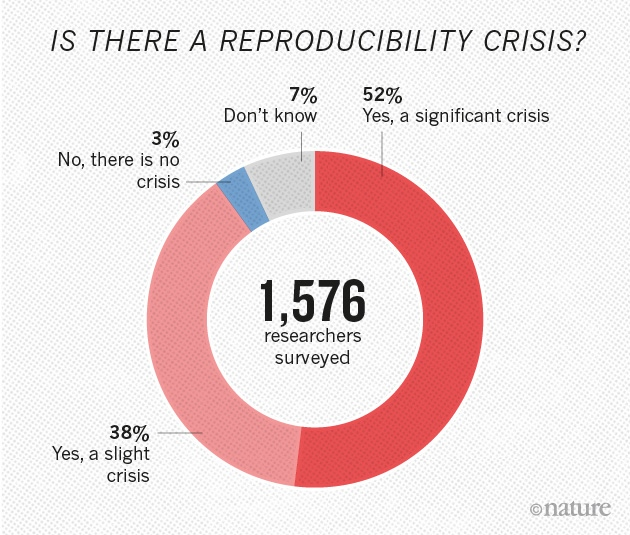
\includegraphics[height=.7\textheight]{figures/reproducibility-graphic-online1.jpeg}
        \caption{Is there a reproducibility crisis? \cite{Baker2016-cf}}
        \label{fig:Baker2016}
  \end{figure}
\end{frame}

\begin{frame}{Lost data}
 \begin{figure}[H]
    \centering
        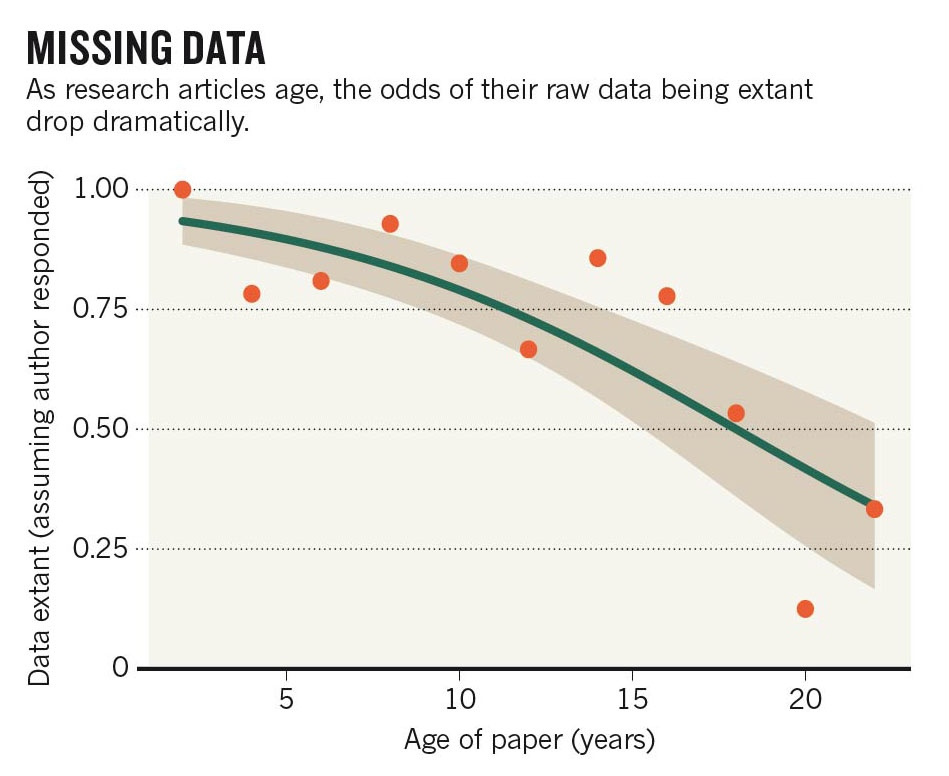
\includegraphics[height=.75\textheight]{figures/Missing-Data.png}
        \caption{\cite{Vines2014-zr}}
        \label{fig:vines2014}
 \end{figure}
\end{frame}

\begin{frame}{Calls for rigour and transparency}
  Manifestos, statements, and guides to good practice:
    \begin{itemize}[label=\textbullet]
        \item \textbf{OECD Priniples and Guidelines for Access to Research Data} \cite{Oecd2007-vi}.
        \item \textbf{Findable, Accessible, Interoperable, and Reusable (FAIR) data} \cite{Wilkinson2016-mr, Go-fair2017-vs}.
        \item \textbf{Transparency and Openness Promotion (TOP) guidelines} \cite{Nosek2015-wm, Cos2019-mr}.
        \item \textbf{Data transparency toolkit} \cite{Perkel2018-rw} provides a snapshot of emerging good practice.
    \end{itemize}
\end{frame}

\begin{frame}{From guidelines to mandates}
  Mandates for transparency or reproducibility:
    \begin{itemize}[label=\textbullet]
        \item \textbf{Nature}: Transparency Upgrade \cite{Nature2017-lq}.
        \item \textbf{Nature}: FAIR data in Earth science \cite{Nature2019-ng}.
        \item \textbf{Copernicus}: FAIR data in atmospheric sciences \cite{Van_Edig2018-bu}.
        \item \textbf{TOP Guidelines} signatories include publishers representing \textbf{1000+ journals}, as well as professional organisations and \textbf{private foundations}  \cite{Cos2019-mr}.
    \end{itemize}
\end{frame}

% https://tex.stackexchange.com/a/2292/5483
% https://ctan.org/pkg/enumitem?lang=en

\begin{frame}{Level 2 TOP Guidelines for authors (excerpt)}
  
    \begin{enumerate}[label=\arabic*.]
        \setcounter{enumi}{1}
        % This increments the enumerate counter by 1.
        
        \item Authors using original data must:
        \begin{enumerate}[label=\alph*.]
            \item \textbf{make the data available} at a trusted digital repository [...]
            \item include all variables, treatment conditions, and observations described in the manuscript.
            \item \textbf{provide a full account of the procedures} used to collect, preprocess, clean, or generate the data.
            \item \textbf{provide program code}, scripts, codebooks, and other documentation sufficient to precisely reproduce all published results.
            \item \textbf{provide research materials and description of procedures} necessary to conduct an independent replication of the research.
        \end{enumerate}
    \end{enumerate}
    (Emphasis added) \cite{Osf2014-pf}
\end{frame}

\begin{frame}{Scalable approaches to data \& analysis}
  \begin{figure}[H]
    \centering
        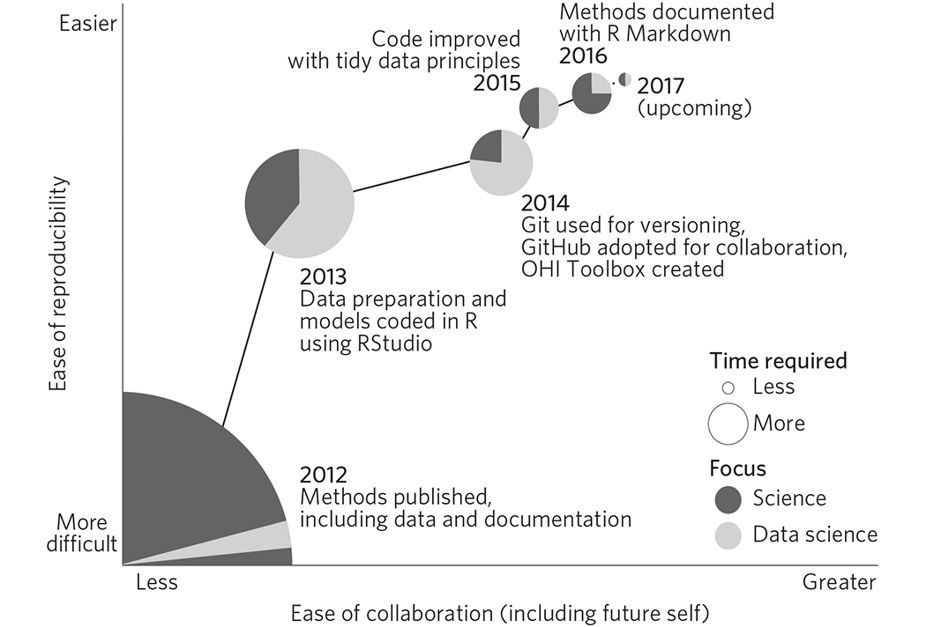
\includegraphics[height=.7\textheight]{figures/Ocean-Health-Index.jpg}
        \caption{Better science in less time, illustrated by the Ocean Health Index project. \cite{Stewart_Lowndes2017-lj}}
        \label{fig:stewart_lowndes}
  \end{figure}
\end{frame}

\begin{frame}{Carpentries as fundamental training}
     The \textbf{legal, ethical, publisher, and funder compliance environment is changing} so fast that training addressed at compliance alone quickly becomes outdated, and learning by rote becomes unworkable (or at least very inefficient). \par
     To meet these challenges, \textbf{research training needs to include fundamental digital skills} that provide a basis to meet rapidly changing expectations. \par
     \textbf{Reproducibility and transparency} have irreducible technological demands. \par
     \textbf{Robust, high-impact research} addressing `grand challenges'  requires data synthesis and scalable approaches to research have  irreducible technological demands.
\end{frame}


\section{What is Carpentries training?}

\begin{frame}{Aims of Carpentries training}
  \textbf{Software Carpentry} \cite{The_Carpentries2019-ej}
  \begin{itemize}[label=\textbullet]
    \item `teach[es] researchers the computing skills they need to get more done in less time and with less pain'
    \item `covers the core skills needed to be productive in a small research team'
  \end{itemize}
  \textbf{Data Carpentry} \cite{The_Carpentries2019-aa}
  \begin{itemize}
    \item `covers the core skills needed to be productive in a small research team'
    \item `high-quality, domain-specific training covering the full lifecycle of data-driven research'
    \item `\textit{Our initial target audience is learners who have little to no prior computational experience}' (emphasis in original)
  \end{itemize}
\end{frame}

\begin{frame}{Delivery of Carpentries training}
  \begin{itemize}[label=\textbullet]
    \item \textbf{Two-day workshops} run by (volunteer) certified instructors, with co-instructors or helpers to ensure sufficient support for learners.
    \item Beginner workshops \textbf{assume no experience}.
    \item Beginner workshops \textbf{build confidence}.
    \item Workshops follow the principal of '\textbf{no one left behind}'.
    \item Workshops are \textbf{community maintained an openly licensed}.
    \item Proven success: Over \textbf{32,000 learners} have been trained at more than \textbf{1,200 workshops} since 2012.
    \item Recommended by (e.g.) 'A toolkit for data transparency' in \textit{Nature} \cite{Perkel2018-rw}
  \end{itemize}
\end{frame}

\section{Carpentries training at Macquarie}

\begin{frame}{Workshops and learners}
  \begin{itemize}[label=\textbullet]
    \item \textbf{12 Workshops} offered since mid-2017.
    \item Over \textbf{500 learners} trained.
    \item Pool of about \textbf{20 instructors} developed.
    \item First '\textbf{Instructor trainers}' certified in 2019, so we can train our own instructors (and provide that service more broadly).
    \item In 2019, \textbf{Data Carpentry integrated into two Masters of Research units}, one in Science and one in Arts.
  \end{itemize}
\end{frame}

\begin{frame}{Reflection on Carpentries training}
  \begin{itemize}[label=\textbullet]
    \item Effectively \textbf{trains researchers beyond compliance}.
    \item \textbf{Well received in STEM} disciplines - we need to \textbf{deliver more} and engage in routine outreach.
    \item In \textbf{HASS disciplines}, response ranges from \textbf{indifference to hostility} (few HASS learners; students in the Arts MRes unit rebelled) - we need to \textbf{change hearts and minds}.
    \item \textbf{Community of practice} emerging: `\textbf{Pipeline}' from learners to helpers to instructors, \textbf{user groups} spawned / strengthened.
    \item \textbf{Volunteer basis of operation may not be sustainable}.
  \end{itemize}
\end{frame}

\begin{frame}{Changes coming to HASS disciplines}
  HASS HDR students (and researchers) unprepared for the emerging world of Open Scholarship, which demands technical skills:
    \begin{itemize}[label=\textbullet]
        \item \textbf{American Journal of Political Science} requires (and tests) data and code \cite{Jacoby2017-lw, Ajps2015-ex}.
        \item \textbf{All European Academies (allea)} E-Humanities working group \cite{Allea2019-wy} has issued an Open Consultation on `Sustainable and FAIR Data Sharing in the Humanities' \cite{Allea2019-aw}.
        \item \textbf{Allea} seeks to address the imperatives of the `\textbf{Open Science agenda}' across Humanities and Social Sciences, and `facilitate the adoption of Open Science across the Humanities'.
        \item \textbf{Research Data Alliance} (RDA) has an 'Ambassador for the Humanities' and is examining how RDA standards and outputs can apply to humanities disciplines \cite{Rda2019-wc}.
    \end{itemize}
\end{frame}

\begin{frame}{Thank you!}

% This presentation is available at:
% \texttt{https://osf.io/...}

This presentation is available at: \texttt{https://github.com/saross/MQ-SWC/releases/tag/v1.0}

This work is licensed under a Creative Commons Attribution 4.0 International License.

\end{frame}

% \bibliographystyle{apalike}

% Adding the option 'allowframebreaks' allows the contents of the slide to be expanded in more than one slide.
% The "1" comes from the outer theme"

\section{References}

\begin{multicols}{2}[]
\bibliography{references}
\bibliographystyle{apalike}
\end{multicols}


% \begin{frame}[allowframebreaks]{References}
  
%   \bibliography{references}
%   \bibliographystyle{apalike}
% \end{frame}

\end{document}